\begin{frame}{Timed Automata}

  $$\mathcal{A}=(A,C,\mathit{inv},\mathit{guard},\mathit{reset})$$
  \vfill
  \begin{center}
    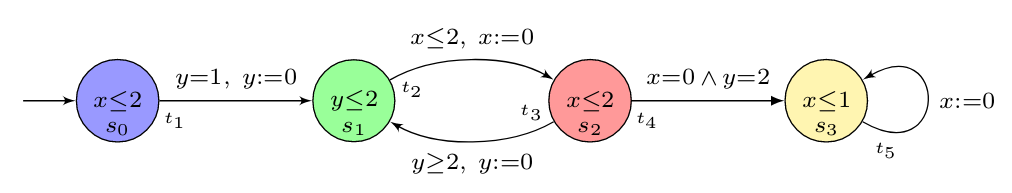
\includegraphics[scale=0.3]{timed.png}
  \end{center}
  \vfill
  \textbf{Time-event sequence}: $t_1~a_1\dots t_n~a_n~\in (\mathbb{R}\times\Sigma)^*$\\
  \textbf{Timed Language}: subset of $(\mathbb{R}\times\Sigma)^*$\\
  \textbf{Complement of $L$}: $(\mathbb{R}\times\Sigma)^* - L$
  
\end{frame}


\begin{frame}{Deterministic Timed Automata}

  \begin{block}{Determinism}
    \begin{itemize}
    \item Only one start state
    \item 2 transitions from the same state with the same label ($\in\Sigma$) have mutually exclusive clock constraints
    \end{itemize}
  \end{block}
  \vfill
  \begin{block}{Property}
    At most one run for one time-event sequence.
  \end{block}

\end{frame}


\begin{frame}{Known Results on Timed Automata}

  \begin{alertblock}{Regular timed languages}
    Regular timed languages are not closed under complementation.\\
    They are closed under union and intersection.
    {\color{red} Give an example?}
  \end{alertblock}
  \vfill
  \begin{alertblock}{Undecidability of the universality problem}
    Given timed automaton $\mathcal{A}$, it is undecidable whether $$\mathcal{L(A)}=(\mathbb{R}\times\Sigma)^*.$$
  \end{alertblock}
\end{frame}


